
\aaa{Orthogonal Projections}
\[defi]{[equivalent definitions]A projection $P=P^2$ is called \x{orthogonal projection} if $P^T=P$}
\[defi]{[equivalent definitions]A projection $P=P^2$ is called \x{orthogonal projection} if $\ker(P) \perp \im(P)$}
We need to show for $P^2=P$, that $P^T=P$ ⟺   $\ker(P) \perp \im(P)$.
\a\aa
Since always $“col“(P^T)\perp “null“(P)$, if $P^T = P$, then $“col“(P) = “col“(P^T)\perp “null“(P)$.
\vfill
On the other hand, if $\ker(P)\perp \im(P)$, then 
$$\im(I-P)=\ker(P)\perp\im(P),$$ so
$$
(I-P)^TP = 0.
$$
This implies $P=P^TP$, transpose this expression we get 
$$P^T=(P^TP)^T=P^TP = P.$$
\a{Just a joke}
Fake proof of $P^T=P$  ⟺    $“Ker“(P) \perp “Im“(P) $


``being orthogonal" = ``being symmetric"
\vfill
\[columns]{
\co5
\[zz]{
\draw[ultra thick](0,0)--(4,0);
\draw[ultra thick](2,0)--(2,4);
}

Orthogonal
\co5
\[zz]{
\draw[ultra thick](0,4)--(4,4);
\draw[ultra thick](2,0)--(2,4);
}

Symmetric
}
\aaa





\aaa{Uniqueness of Orthogonal Complement}
\[lem]{For any vector $\vec v$, $\vec v^T \vec v=0$ implies $\vec v=\vec 0$}

$$
x_1^2+...+x_n^2 = 0  ⟹  x_1=x_2=...=x_n=0.
$$
\a\aa
\[thm]{[Extremely important theorem]For any real number matrix $A$, if $A^TA=0$, then $A=0$.}
$$
( ∀ i, e_i^T A^TAe_i=0 ⟹  Ae_i =\vec 0 ) ⟹  A=0.
$$
\[prop]{For any real number matrix $A$, $“Null“(A^TA)=“Null“(A)$}

For sure $“Null“(A^TA) ⊇  “Null“(A)$, 

If $A^TA\vec v=0$, then $\vec v^TA^TA\vec v=0$, then $A\vec v=0$ then $\vec v ∈ “Null“(A)$.
\a\aa
\[thm]{[Orthogonal Complement is unique] For any subspace $W$, there is only one \x{orthogonal} projection $P$ with $“Im“(P)=W$. }
Let $P=P^T=P^2$ and $Q=Q^T=Q^2$ be projections such that $W = \im(P)=\im(Q)$.  
$$
“Im“(P) ⊇ “Im“(Q) ⟹  PQ = Q, ␣ “Im“(Q) ⊇ “Im“(P) ⟹  QP = P.
$$

$$
(P-Q)^T(P-Q)
$$$$=(P-Q)(P-Q) 
$$$$=P^2 -PQ -QP - Q^2 
$$$$= P-Q-P-Q = 0.
$$
So $P-Q = 0$.
\a\aa
\[cor]{The orthogonal complement has to be unique.
}
There is a unique orthogonal projection $P$ for $W ⊆  ℝ^n$.

If $U$ is orthogonal compment of $W$, then $U \perp W$ implies $U ⊆ “ker(P)“$.

$U$ has to have dimension $“dim“(U) = n - “dim“(W) = “dim ker“(P)$. 

So $U = “ker“(P)$

$P$ is unique, $“ker“(P)$ is unique, so $U$ is unique.

\a{Notation for Orthogonal Complement}
\[defi]{For a vector space $W ⊆  ℝ^n$, we denote its orthogonal complement by $W^\perp$.}

Let $P$ be the orthogonal projection that is uniquely determined by $W$, for any vector $\vec v$, we can always decompose
$$
\vec v = \underbrace{ P \vec v}_{ ∈ W} +\underbrace{ (I-P)\vec v}_{ ∈ W^\perp}
$$
\a\aa
\[prop]{For any vector $\vec v$ such that $\vec v^T\vec w=0$ for all $\vec w ∈ W$, then $\vec v ∈ W^\perp$}
\textbf{Proof}: For any vector $\vec e$, we have
$$
\vec e^TP\vec v = \vec e^TP^T \vec v = \underbrace{(P\vec e)^T}_{∈ W}\vec v = 0.
$$
So $P\vec v=0$. Therefore, $(I-P)\vec v=\vec v$, then $\vec v ∈ “Im“(I-P) = W^\perp$.
\a\aa
\[rem]{This implies that $W^\perp = \{\vec v: \vec v^T\vec w=0 “for all “\vec w ∈ W \}$
Put 

$$
P = \m{\vec w_1}\cdots{\vec w_n}.
$$

$$
W^\perp = \ker(P) \xequal{P=P^T} \ker(P^T)= \{\vec v: P^T\vec v=\vec 0\} 
$$
$$
\xequal{} \{\vec v:(\vec w_i)^T\vec v=0 “ for all “1≤i≤n\}
$$
$$
\xequal{} \{\vec v:\vec w^T\vec v=0 “ for all “ \vec w ∈ “Im“(P)\}
$$
$$
\xequal{} \{\vec v:\vec w^T\vec v=0 “ for all “ \vec w ∈ W\}
$$
In one words, $W^\perp$ is the subset of \x{all} vectors orthogonal to $W$.
}

%\a\aa
%\[prop]{For any matrix $A$, we have $“Col“(A)=“Col“(AA^T)$}
%Because $“Col“(A) = “Null“(A^T)^\perp$ and $“Col“(AA^T) = “Null“(AA^T)^\perp$. Since $“Null“(A^T) = “Null“(AA^T)$, we have $“Null“(A^T)^\perp = “Null“(AA^T)^\perp$
%
%\a\aa
%
%$$A^T = \m{r_1}{\cdots}{r_m}.$$ 
%
%$$
%AA^T = \m{Ar_1}{\cdots}{Ar_m}.
%$$
%
%Therfore, $“span“\{Ar_1, Ar_2,..., Ar_m\} = “Col“(A)$
%
%
%As a linear transformation, the matrix $A$ maps its row space to its column space.
%%\a\aa
%%\[thm]{The orthogonal complement is unique.}


\a\aa
The intuitive picture for orthogonal complement
\[tikzpicture]{[scale=0.5]

%	\draw[ultra thick,red] (-6,0)--(6,0) node[right]{$U_1$};
	\draw[ultra thick,red] (0,-4)--(0,0);
	\draw[fill=green,opacity=0.5] (-7,-1)--(1,-1)--(7,1) node[right]{$W_1$} --(-1,1)--(-7,-1);
        \draw[ultra thick,red] (0,0)--(0,5) node[above]{$W_2$};
%	\draw[ultra thick,red] (-6,-2)--(6,2) node [right]{$U_2$};
	\draw[fill=red] (0,0) circle[radius=0.1] node[right]{$\vec 0$};
	}


\a{Formula for orthogonal projection}
\[prop]{
Let $W=“Col“(A)$ for some matrix $A$ with \li columns. Then $W^\perp = “Null“(A^T)$. 
$$
P := A(A^TA)^{-1}A^T
$$
 is an \x{orthogonal projection} with $“Im“(P)=“Im“(A)$ and $“Null“(P)=“Null“(A^T) = W^\perp$.
}
\[itemize]{
\item (being projection $P^2=P$)A more general formula: $P=A(BA)^{-1}B$ is a projection with $“Null“(P)=“Null“(B)$ and $“Col“(P)=“Col“(A)$. 
\vfill
\item (being orthogonal)$P^T = (A(BA)^{-1}B)^T = B^T (A^TB^T)A^T$. If $B=A^T$, then $P=P^T$.
\vfill
\item $A^TA$ is invertible since $“Null“(A^TA)=“Null(A)“=0$
}
\a\aa
A special case for one-dimensional space $“Im“(A) =“Col“(\vec v)$ for one vector $\vec v$.
\vfill
 There is a unique rank-1 orthogonal projection given by 
$$P = v(v^Tv)^{-1}v^T  ␣  = \frac{vv^T}{v^Tv}$$
 all rank-1 orthogoal proejctions arises in this way.

\a\aa
\exe Suppose $W$ is a subspace in $ℝ^3$ spanned by 
$$
\m 1,1,1. ␣ \m 1,0,{-1}.
$$
Find the orthogonal projection to this space, and find a basis of its orthogonal complement.
\a\aa

\sol The orthogonal complement is just the kernel of the orthogonal projection to it. We find orthogonal projection using formula. Note that

$$
W = “Col“ \underbrace{\m11,10,1{-1}.}_A
$$
An orthogonal projection can be formulated as 
$$
P = \underbrace{A}_{“for column space“}(A^TA)^{-1}\underbrace{A^T}_{“ for null space “}
$$
\a\aa
A calculation implies that
$$
A(A^TA)^{-1}A^T
=
\m11,10,1{-1}.\left(\m111,10{-1}.\m11,10,1{-1}.\right)^{-1}\m111,10{-1}.
$$
$$
=\m11,10,1{-1}.\m30,02.^{-1}\m111,10{-1}.
$$
$$
=\m11,10,1{-1}.\m{\frac13}{\frac13}{\frac13},{\frac12}0{-\frac12}.
$$
$$
=\m{\frac56}{\frac13}{-\frac16},
{\frac13}{\frac13}{\frac13},
{\frac16}{\frac13}{\frac56}.
$$
This is the orthogonal projection we are looking for.%\x{This matrix is symmetric, and has trace 2.}
\a\aa
Now that we have find 
$$
P = \m{\frac56}{\frac13}{-\frac16},
{\frac13}{\frac13}{\frac13},
{-\frac16}{\frac13}{\frac56}.
$$
The orthogonal complement is $\ker(P)=“Im“(I-P)$. Just calculate
$$
I - P = \m{\frac16}{-\frac13}{\frac16},
{-\frac13}{\frac23}{-\frac13},
{\frac16}{-\frac13}{\frac16}.
$$
Since it is trace(rank) 1 projection, any column is a basis for its image. So a basis of $W^\perp$ can be
$$
\m 1,{-2},1.
$$
\a\aa
\sol Yet there is another solution. We may find orthogonal complement first before determine the orthogonal projeciton. $W=“col“\m11,10,1{-1}.$
So its orthogonal complement is
$$
“null“\m111,10{-1}.
$$
Solve the equation, we have
$$
W^\perp = “null“\m111,10{-1}. = “Col“\m1,{-2},1.
$$
\a\aa
To find orthogonal projection to $W$. We found orthogonal projection to $W^\perp$ first.
$$
P_W = P_{W^\perp}=\m1,{-2},1.\left(\m1{-2}1.\m1,{-2},1.\right)^{-1}\m1{-2}1.
=
\m1,{-2},1.\frac16\m1{-2}1.
$$
$$
=\m{\frac16}{-\frac13}{\frac16},
{-\frac13}{\frac23}{-\frac13},
{\frac16}{-\frac13}{\frac16}.
$$

So the projection to $W$ is 
$$I-P_{W^\perp} = \m{\frac56}{\frac13}{-\frac16},
{\frac13}{\frac13}{\frac13},
{-\frac16}{\frac13}{\frac56}.$$

\aaa





\aaa{Distance and Orthogonal Projections}
In order to find the distance of a point to a subspace, we may decompose a vector into two component $\vec v=\vec v^\parallel +\vec v^\perp$, with $\vec v^\parallel\in W$ and $\vec v^\perp\in W^\perp$.
\[columns]{\co5
\[zz]{
\draw[->,ultra thick] (0,0)--(1,2) node[right]{$\vec v$};
\draw[thick] (-3,0)--(3,0) node[right]{$W$};
\dian12
%\draw[dotted,ultra thick] (0,0)--(0,2);
}
\co 5
\[zz]{
\draw[->,ultra thick] (0,0)--(1,2);
\draw[thick] (-3,0)--(3,0) node[right]{$W$};
\draw[->,ultra thick,red] (0,0)--(0,2) node[left]{$\vec v^\perp$};
\draw[dotted,ultra thick,blue] (0,2)--(1,2);
\draw[->,ultra thick,blue] (0,0)--(1,0) node[below]{$\vec v^\parallel$};
\draw[dotted,ultra thick,blue] (1,0)--(1,2);
}
}
Let $P$ be the orthogonal projection associated to $W$, we may write
$$ \vec v^\parallel = P\vec v $$
$$ \vec v^\perp = (I-P)\vec v $$
For any $\vec w ∈ W$, we have $\vec w - \vec v^\parallel ∈ W$ therefore
$$ (\vec v^\perp)^T(\vec w - \vec v^\parallel)=0.  $$
$$ (\vec w - \vec v^\parallel)^T(\vec v^\perp)=0.  $$
\a\aa
\[zz]{
\draw[->,ultra thick] (0,0)--(1,2);
\draw[thick] (-3,0)--(3,0) node[right]{$W$};
\draw[->,ultra thick,red] (0,0)--(0,2) node[left]{$\vec v^\perp$};
\draw[dotted,ultra thick,blue] (0,2)--(1,2);
\draw[->,ultra thick,blue] (0,0)--(1,0) node[below]{$\vec v^\parallel$};
\draw[dotted,ultra thick,blue] (1,0)--(1,2);
}


$$(\vec v-\vec w)^T(\vec v-\vec w)$$
$$=(\vec v^\perp - (\vec w - \vec v^\parallel))^T(\vec v^\perp - (\vec w - \vec v^\parallel))$$
$$
=(\vec v^\perp)^T(\vec v^\perp) + (\vec w - \vec v^\parallel)^T(\vec w - \vec v^\parallel)
$$

This implies that

$$
||\vec v-\vec w||² = ||\vec v^\parallel-\vec w||²+||\vec v^\perp||^2
$$


\a\aa
$$
||\vec v-\vec w||² = \underbrace{||\vec v^\parallel-\vec w||²}_{≥ 0}+||\vec v^\perp||^2
$$
$$
\min_{\vec w ∈ W} ||\vec v-\vec w||² = ||\vec v^\perp||^2
$$
The minimal such choice is $\vec w = \vec v^\parallel$.

In other words, the orthogonal projection is the point on the plane with minimal distance to the given point. We define this distance as distance of a point to the subspace.
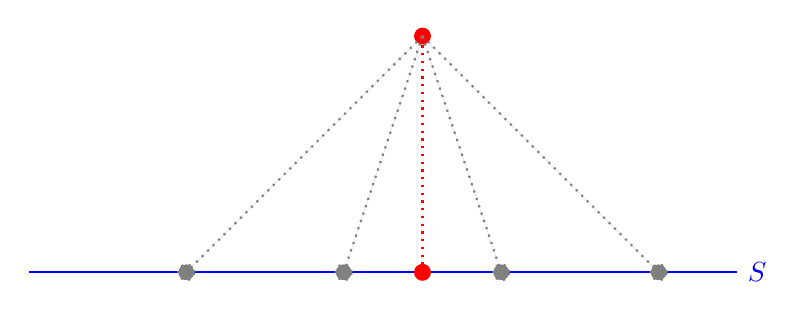
\begin{tikzpicture}
    \draw[ thick,blue](-3,0)--(6,0) node[right] {$S$};
 %   \draw[->, ultra thick, red](0,0)--(2,0) node[below] {$\comp{\vv}{\ww}$};
 %   \draw[->, thick,blue](0,0)--(2,3) node[right] {$\vv$};
	\draw[fill,red] (2,3) circle[radius=0.1];
	\draw[fill,red] (2,0) circle[radius=0.1];
    \draw[dotted, thick,red](2,0)--(2,3);
    \draw[dotted, thick,gray,fill=gray](2,3)--(3,0) circle[radius=0.1];
    \draw[dotted, thick,gray,fill=gray](2,3)--(1,0) circle[radius=0.1];
    \draw[dotted, thick,gray,fill=gray](2,3)--(-1,0) circle[radius=0.1];
    \draw[dotted, thick,gray,fill=gray](2,3)--(5,0) circle[radius=0.1];
\end{tikzpicture}


\a\aa
\exe Suppose $W ⊆  ℝ^3$ is given by the equation
$$
x+2y+3z = 0
$$
Please find the formula of the distance of the point $(x_0,y_0,z_0)$ to the plane and find its closest point on the plane, in terms of $x_0,y_0,z_0$.

\vfill
\[z]{[scale=0.4]
\draw[fill=pink](-12,-2)--(2,-2)--(12,2)--(-2,2)--(-12,-2);
%\draw[blue,ultra thick,->](0,0)--(6,0);
%\draw[blue,ultra thick,->](0,0)--(2.5,1);
%\draw[purple, ultra thick,->](0,0)--(-4,0);
%\draw[purple, ultra thick,->]
%(0,0)--(-3,-1.2);
%\draw[orange, ultra thick,dotted](-7,-1.2)--(-4,0) (-7,-1.2)--(-3,-1.2);
\draw[red, ultra thick,->](0,0)--(-7,-1.2);
\draw[ultra thick,->](0,0)--(-7,4) node[left]{$(x_0,y_0,z_0)$};
\draw[ultra thick,dotted](-7,-1.2)--(-7,4);
}


\a\aa
\sol. First, we want to find out the projection to $W^\perp$. Let 
$$
A = \m123.
$$
Then $“Col“(A^T) = W^\perp$
The unique orthogonal projection mapping to $W^\perp$ is given by
$$
P = A^T(AA^T)^{-1}A  = \frac1{14}\m1,2,3.\m123.
$$

$$
P\m{x_0},{y_0},{z_0}. = \frac1{14}\m1,2,3.\m123.\m{x_0},{y_0},{z_0}. = \frac{x_0+2y_0+3z_0}{14}\cdot \m1,2,3.
$$
\a\aa
Therefore, the distance is given by
$$
||P\vec v|| = \frac{\sqrt{14}}{14}\cdot |x_0+2y_0+3z_0|.
$$

Then , the orthogonal projection to $W$ is given by $I-P$. So
$$
\vec v ↦  (I-P)\vec v = \frac1{14}\m{13}{-2}{-3},{-2}{10}{-6},{-3}{-6}5.\m{x_0},{y_0},{z_0}.
$$
is the formula of the point in $W$ that is closest to $\vec v$.
\aaa
